\documentclass[11pt,a4paper]{article}
\usepackage[T1]{fontenc}
\usepackage{lmodern}
\usepackage[margin=1.7cm,top=2.2cm,bottom=2cm]{geometry}
\usepackage{graphicx}
\usepackage[table]{xcolor}
\usepackage{tikz}
\usepackage{fancyhdr}
\usepackage[most]{tcolorbox}
\usepackage{microtype}
\definecolor{navy}{RGB}{21,45,99}
\definecolor{ocean}{RGB}{28,97,158}
\definecolor{aqua}{RGB}{0,142,150}
\definecolor{sky}{RGB}{235,243,252}
\definecolor{ink}{RGB}{40,40,50}
\renewcommand{\familydefault}{\sfdefault}
\color{ink}
\pagestyle{fancy}\fancyhf{}
\renewcommand{\headrulewidth}{0pt}
\fancyhead[L]{\small\color{navy}\textbf{Module 1: Foundations of Network Security} \,\textbar\, Speaker Notes}
\fancyhead[R]{
\includegraphics[height=0.75cm]{../au_logo.png}}
\fancyfoot[C]{\small\color{ocean}\thepage}
\setlength{\parindent}{0pt}
\newtcolorbox{slidebox}[3]{enhanced,breakable=false,colback=white,colframe=ocean,boxrule=0.6pt,arc=2mm,
  left=3mm,right=3mm,top=2mm,bottom=2mm,
  title={\textbf{Slide #1}\;\,|\;\,#2\quad\normalfont\small(about #3 seconds)},
  fonttitle=\sffamily\color{white},colbacktitle=navy,attach boxed title to top left={yshift=-2mm,xshift=3mm},
  boxed title style={arc=1.5mm,colback=navy},before skip=5mm,after skip=3mm}
\begin{document}
\thispagestyle{empty}
\begin{tikzpicture}[remember picture,overlay]
  \fill[navy] (current page.north west) rectangle ([yshift=-9.5cm]current page.north east);
  \fill[aqua] ([yshift=-9.5cm]current page.north west) rectangle ([yshift=-9.7cm]current page.north east);
  \node[anchor=north east] at ([xshift=-1.5cm,yshift=-1.2cm]current page.north east) {
\includegraphics[height=2.4cm]{../au_logo.png}};
  \node[anchor=west,white,font=\large] at ([xshift=1.8cm,yshift=-2.2cm]current page.north west) {NETWORK SECURITY \,\textbar\, MODULE 1};
  \node[anchor=west,white,font=\fontsize{30}{36}\selectfont\bfseries] at ([xshift=1.8cm,yshift=-4.2cm]current page.north west) {Speaker Notes};
  \node[anchor=west,white,font=\Large] at ([xshift=1.8cm,yshift=-5.6cm]current page.north west) {Foundations of Network Security};
  \node[anchor=west,white,font=\normalsize,align=left] at ([xshift=1.8cm,yshift=-7.2cm]current page.north west)
    {Lesson 1: Introduction to Network Security\\Lesson 2: Network Models};
\end{tikzpicture}
\vspace*{8.6cm}

\begin{tcolorbox}[colback=sky,colframe=ocean,arc=2mm,title=\textbf{How to use these notes},fonttitle=\sffamily]
\begin{itemize}\setlength{\itemsep}{3pt}
  \item There is \textbf{one note for each of the 52 slides}, in the same order as \texttt{module1.pdf}. A small picture of the slide sits beside each note.
  \item The notes are written \textbf{from teacher to students}: speak them as they are, or use them as a guide in your own words.
  \item Each note is about \textbf{100--112 words}, which takes roughly \textbf{45--50 seconds} at a steady classroom pace of about 135 words per minute. The estimate for each slide is shown in its title bar.
  \item Phrases such as ``look at the diagram'' tell you when to point at the slide.
\end{itemize}
\end{tcolorbox}

\vspace{4mm}
\begin{center}
\renewcommand{\arraystretch}{1.5}
\begin{tabular}{>{\columncolor{navy}\color{white}\bfseries}l >{\columncolor{sky}}l}
Slides & 52 \\
Total words & 5,471 \\
Estimated talking time & about 41 minutes (without pauses or questions) \\
Lesson 1 & slides 3--31 \\
Lesson 2 & slides 32--52 \\
\end{tabular}
\end{center}
\newpage
\begin{slidebox}{1}{Title: Foundations of Network Security}{47}
\begin{minipage}[t]{0.40\linewidth}\vspace{0pt}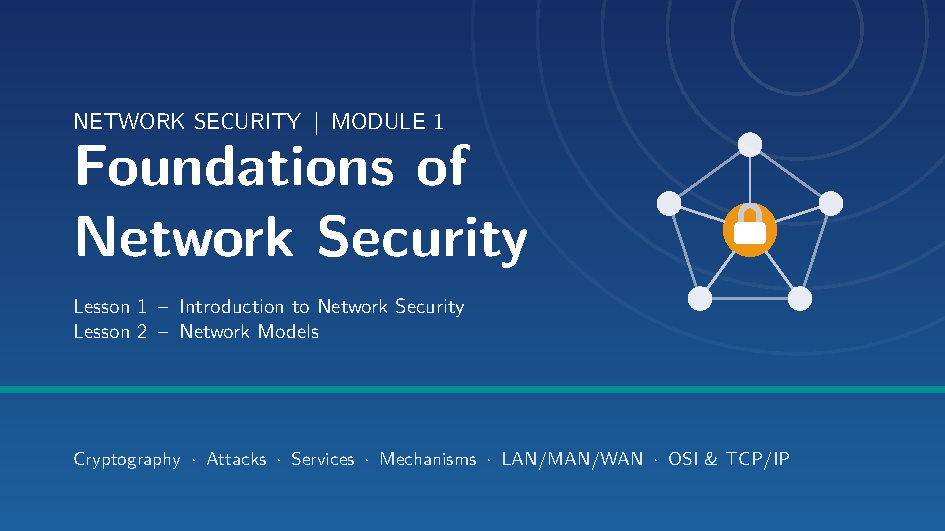
\includegraphics[width=\linewidth,page=1]{../module1.pdf}\end{minipage}\hfill
\begin{minipage}[t]{0.57\linewidth}\vspace{0pt}\small\linespread{1.1}\selectfont Good morning, everyone, and welcome to our Network Security course. Today we begin with Module 1, Foundations of Network Security. This module brings together two lessons from your study material. Lesson 1 is the Introduction to Network Security, and Lesson 2 is about Network Models. Think of this module as laying the foundation of a building: everything we study later, from ciphers to firewalls, stands on the ideas we learn today. Along the way you will meet words like cryptography, attacks, services, mechanisms, LAN, WAN, OSI and TCP/IP. Do not worry if these sound new; by the end, each will make sense. Let us get started.\end{minipage}
\end{slidebox}
\begin{slidebox}{2}{Roadmap of This Module}{48}
\begin{minipage}[t]{0.40\linewidth}\vspace{0pt}\includegraphics[width=\linewidth,page=2]{../module1.pdf}\end{minipage}\hfill
\begin{minipage}[t]{0.57\linewidth}\vspace{0pt}\small\linespread{1.1}\selectfont Before we dive in, let me show you our roadmap, so you always know where we are. On the left are the first four stops, all from Lesson 1. We start by asking why security matters at all, then learn the basics of cryptology, then the three aspects of security, which are attacks, services and mechanisms, and then the four main types of attack. On the right, we continue with cryptographic systems and how attackers try to break them. The last two stops come from Lesson 2: the different categories of networks, and finally the layered models, OSI and TCP/IP. Keep this map in mind as we move.\end{minipage}
\end{slidebox}
\begin{slidebox}{3}{Lesson 1: Introduction to Network Security}{47}
\begin{minipage}[t]{0.40\linewidth}\vspace{0pt}\includegraphics[width=\linewidth,page=3]{../module1.pdf}\end{minipage}\hfill
\begin{minipage}[t]{0.57\linewidth}\vspace{0pt}\small\linespread{1.1}\selectfont We now begin Lesson 1, Introduction to Network Security. In this lesson our aim is simple but very important. First, we want to understand why information needs protection in the first place. Second, we will define the three security goals that every system tries to achieve. Third, we will study the attacks that threaten those goals, and the services and mechanisms that defend against them. Finally, we will get our first look at cryptography, the most common tool for providing security, and at cryptanalysis, the art of breaking it. Please pay attention to the definitions in this lesson, because they are frequently asked in examinations.\end{minipage}
\end{slidebox}
\begin{slidebox}{4}{We Live in the Information Age}{48}
\begin{minipage}[t]{0.40\linewidth}\vspace{0pt}\includegraphics[width=\linewidth,page=4]{../module1.pdf}\end{minipage}\hfill
\begin{minipage}[t]{0.57\linewidth}\vspace{0pt}\small\linespread{1.1}\selectfont Look at the diagram on the left. In the middle is the Internet, and around it you can see the things all of you do every day: shopping online, sending e-mail, browsing the World Wide Web, banking, and chatting with friends. The Internet has truly changed our daily life. But here is the catch. Because we depend on it so much, and anyone can join this open forum, it has also created serious security problems. When you shop online, you want your conversation kept confidential. You want to be sure the shop is authentic. And when you send a request to your bank, you want its integrity preserved.\end{minipage}
\end{slidebox}
\begin{slidebox}{5}{Information Is an Asset}{50}
\begin{minipage}[t]{0.40\linewidth}\vspace{0pt}\includegraphics[width=\linewidth,page=5]{../module1.pdf}\end{minipage}\hfill
\begin{minipage}[t]{0.57\linewidth}\vspace{0pt}\small\linespread{1.1}\selectfont Let us see how the need for security has grown over time. In the first era, information lived in physical files. To protect it, we locked the cabinet and trusted only a few people. In the second era, information moved into computers. The requirements stayed the same, but now we needed software tools to protect files. In the third era, which is today, information is distributed and sent across networks. So here is the key idea, written in the blue box: information is an asset, just like money or property. It must be hidden from unauthorized access, protected from unauthorized change, and available to authorized users, both when stored and while travelling.\end{minipage}
\end{slidebox}
\begin{slidebox}{6}{Computer, Network and Internet Security}{48}
\begin{minipage}[t]{0.40\linewidth}\vspace{0pt}\includegraphics[width=\linewidth,page=6]{../module1.pdf}\end{minipage}\hfill
\begin{minipage}[t]{0.57\linewidth}\vspace{0pt}\small\linespread{1.1}\selectfont Students often ask me what the difference is between computer security, network security and Internet security. Look at the three circles. The innermost circle is computer security: tools that protect data stored on one computer and keep hackers out. Around it is network security, which protects data while it is being transmitted. The outer circle is Internet security, which covers preventing, detecting and correcting violations across many interconnected networks. But notice the red box. There are no sharp boundaries between them. For example, a virus might arrive on a pen drive or through the network, and once it is inside, computer security tools must deal with it anyway.\end{minipage}
\end{slidebox}
\begin{slidebox}{7}{Two Examples of Security Violations}{49}
\begin{minipage}[t]{0.40\linewidth}\vspace{0pt}\includegraphics[width=\linewidth,page=7]{../module1.pdf}\end{minipage}\hfill
\begin{minipage}[t]{0.57\linewidth}\vspace{0pt}\small\linespread{1.1}\selectfont Here are two examples from your study material. On the left, user A sends a payroll file to user B. User C is not authorized to read it, but C quietly monitors the transmission and captures a copy. Nothing looks wrong to A or B, yet the secret is out. That is a disclosure. On the right, manager D sends an update message to computer E, telling it which users may access the system. Attacker F intercepts that message and adds or deletes names before passing it on. Now the wrong people get access. That is an alteration. Network security is about letting us use the Internet comfortably without such worries.\end{minipage}
\end{slidebox}
\begin{slidebox}{8}{The Three Security Goals: The CIA Triad}{48}
\begin{minipage}[t]{0.40\linewidth}\vspace{0pt}\includegraphics[width=\linewidth,page=8]{../module1.pdf}\end{minipage}\hfill
\begin{minipage}[t]{0.57\linewidth}\vspace{0pt}\small\linespread{1.1}\selectfont Now we come to one of the most important ideas in this entire course, the CIA triad. Please do not confuse it with the intelligence agency. Here C stands for Confidentiality, which means hiding information from unauthorized access. I stands for Integrity, which means protecting information from unauthorized change. A stands for Availability, which means information must be available to authorized people whenever they need it. Look at the triangle: all three goals together keep the lock in the centre secure. Remember the note in the blue box, because it will help you in every later lesson: every attack we study threatens at least one of these three goals.\end{minipage}
\end{slidebox}
\begin{slidebox}{9}{The CIA Goals in Everyday Life}{47}
\begin{minipage}[t]{0.40\linewidth}\vspace{0pt}\includegraphics[width=\linewidth,page=9]{../module1.pdf}\end{minipage}\hfill
\begin{minipage}[t]{0.57\linewidth}\vspace{0pt}\small\linespread{1.1}\selectfont Let me make the CIA goals concrete with everyday examples. For confidentiality, ask yourself: who can read it? Your bank keeps your balance secret, and it is threatened by eavesdropping and traffic analysis. For integrity, ask: has it been changed? A cheque amount must not be altered after you sign it, and integrity is threatened by modification and fabrication. For availability, ask: can I use it right now? An ATM should work even at two in the morning, and availability is threatened by denial of service. If you remember these three simple questions, you will never mix up the three goals in your examination answers.\end{minipage}
\end{slidebox}
\begin{slidebox}{10}{Cryptology = Cryptography + Cryptanalysis}{48}
\begin{minipage}[t]{0.40\linewidth}\vspace{0pt}\includegraphics[width=\linewidth,page=10]{../module1.pdf}\end{minipage}\hfill
\begin{minipage}[t]{0.57\linewidth}\vspace{0pt}\small\linespread{1.1}\selectfont Now let us learn some terminology. The word cryptology comes from Greek: kryptos means hidden, and logos means word. So cryptology is the science of secret messages. It has two branches, as the tree shows. On the left is cryptography, from kryptos and graphein, to write. It is about designing systems to code and decode messages. On the right is cryptanalysis, from kryptos and analyein, to loosen or untie. It is about breaking those systems, that is, recovering messages without knowing the key. Please note the common mistake in the red box: many people use cryptology and cryptography as synonyms, but cryptology is the broader term covering both.\end{minipage}
\end{slidebox}
\begin{slidebox}{11}{The Basic Encryption Model}{48}
\begin{minipage}[t]{0.40\linewidth}\vspace{0pt}\includegraphics[width=\linewidth,page=11]{../module1.pdf}\end{minipage}\hfill
\begin{minipage}[t]{0.57\linewidth}\vspace{0pt}\small\linespread{1.1}\selectfont This diagram is the heart of cryptography, so study it carefully. On the left, the sender has a readable message called plaintext, here ``PAY 100''. It goes into the encryption box, E, together with a secret key K. Out comes ciphertext, a scrambled message like ``SDB 433'' that makes no sense to anyone. At the other end, the decryption box, D, uses the same key to turn the ciphertext back into plaintext. Notice the opponent at the bottom: they can see only the ciphertext. Remember four terms from the bottom of the slide: plaintext, ciphertext, cipher, which is the algorithm, and key, the secret value controlling it.\end{minipage}
\end{slidebox}
\begin{slidebox}{12}{Three Aspects of Information Security}{47}
\begin{minipage}[t]{0.40\linewidth}\vspace{0pt}\includegraphics[width=\linewidth,page=12]{../module1.pdf}\end{minipage}\hfill
\begin{minipage}[t]{0.57\linewidth}\vspace{0pt}\small\linespread{1.1}\selectfont To understand the security needs of any organization, we look at three aspects. First, a security attack is any action that compromises the security of information, such as interruption, interception, modification or fabrication. Second, a security service enhances the security of data processing and transfers; examples are confidentiality, integrity and authentication. Third, a security mechanism is a process designed to detect, prevent or recover from an attack, such as encryption, digital signatures or SSL. Look at the arrows: a service counters an attack, and a service is implemented by one or more mechanisms. These three terms help organizations identify their needs and evaluate security products.\end{minipage}
\end{slidebox}
\begin{slidebox}{13}{An Analogy: Securing a House}{48}
\begin{minipage}[t]{0.40\linewidth}\vspace{0pt}\includegraphics[width=\linewidth,page=13]{../module1.pdf}\end{minipage}\hfill
\begin{minipage}[t]{0.57\linewidth}\vspace{0pt}\small\linespread{1.1}\selectfont If those three terms feel abstract, let me use a simple analogy. Think of your house as the place where your valuable data lives. A burglar breaking in and stealing jewellery is the attack. The rule that only family members may enter is the service; in network terms it is access control or confidentiality. And the locks, alarms and security camera are the mechanisms that actually enforce that rule; in networks, that is encryption and similar tools. So whenever you are confused, ask yourself three questions. What is the burglar doing? What rule do I want? What lock enforces that rule? That is attack, service and mechanism.\end{minipage}
\end{slidebox}
\begin{slidebox}{14}{Services Use Mechanisms}{46}
\begin{minipage}[t]{0.40\linewidth}\vspace{0pt}\includegraphics[width=\linewidth,page=14]{../module1.pdf}\end{minipage}\hfill
\begin{minipage}[t]{0.57\linewidth}\vspace{0pt}\small\linespread{1.1}\selectfont This table connects the services to the mechanisms that provide them. Read it row by row. Confidentiality guarantees that only authorized parties read the data, and it is usually provided by encryption. Integrity guarantees data is not altered in transit, using hashes or digital signatures. Authentication proves the sender is who they claim to be, using signatures or passwords. Non-repudiation means the sender cannot later deny sending, again using a digital signature. Access control limits who uses a resource. Availability keeps the service usable. The key point is at the bottom: a service is what we want, a mechanism is how we get it.\end{minipage}
\end{slidebox}
\begin{slidebox}{15}{Normal Flow of Information}{47}
\begin{minipage}[t]{0.40\linewidth}\vspace{0pt}\includegraphics[width=\linewidth,page=15]{../module1.pdf}\end{minipage}\hfill
\begin{minipage}[t]{0.57\linewidth}\vspace{0pt}\small\linespread{1.1}\selectfont Before we study attacks, we must understand what normal looks like. In the diagram, information flows from a source, which could be a file or a user, to a destination, which is another file or user. The green arrow shows a message travelling safely, and nobody interferes. This is the normal case. Now, each of the four attacks at the bottom of the slide, interruption, interception, modification and fabrication, changes this simple picture in a different way. As we go through the next four slides, keep comparing each diagram with this normal flow. Asking yourself what has changed is the easiest way to remember each attack.\end{minipage}
\end{slidebox}
\begin{slidebox}{16}{Attack 1: Interruption}{45}
\begin{minipage}[t]{0.40\linewidth}\vspace{0pt}\includegraphics[width=\linewidth,page=16]{../module1.pdf}\end{minipage}\hfill
\begin{minipage}[t]{0.57\linewidth}\vspace{0pt}\small\linespread{1.1}\selectfont The first attack is interruption. Look at the diagram: the line from source to destination is cut, and the message never arrives. By definition, in an interruption an asset of the system is destroyed or becomes unavailable or unusable. Which goal does this threaten? Availability, because the information can no longer be used. Some examples: cutting a communication line, destroying a hard disk, disabling a file management system, or flooding a server with fake requests so real users cannot get in, which is called denial of service. So whenever you hear that something has become unavailable, think of interruption and availability together.\end{minipage}
\end{slidebox}
\begin{slidebox}{17}{Attack 2: Interception}{45}
\begin{minipage}[t]{0.40\linewidth}\vspace{0pt}\includegraphics[width=\linewidth,page=17]{../module1.pdf}\end{minipage}\hfill
\begin{minipage}[t]{0.57\linewidth}\vspace{0pt}\small\linespread{1.1}\selectfont The second attack is interception. Notice in the diagram that the message still reaches the destination normally, but an attacker quietly takes a secret copy along the way. By definition, an unauthorized party gains access to an asset. This threatens confidentiality. Examples include wiretapping a line to capture data, illegally copying files or programs, and sniffing passwords on a public Wi-Fi network. Here is something very important to remember: because the original message still arrives unchanged, the sender and receiver often do not even know the attack has happened. That is exactly why interception is so dangerous and so hard to detect.\end{minipage}
\end{slidebox}
\begin{slidebox}{18}{Attack 3: Modification}{46}
\begin{minipage}[t]{0.40\linewidth}\vspace{0pt}\includegraphics[width=\linewidth,page=18]{../module1.pdf}\end{minipage}\hfill
\begin{minipage}[t]{0.57\linewidth}\vspace{0pt}\small\linespread{1.1}\selectfont The third attack is modification. Here the attacker sits in the middle. The source sends ``Pay 100'', the attacker catches it, changes it to ``Pay 900'', and forwards it to the destination, which has no idea anything happened. By definition, an unauthorized party not only gains access to an asset but also tampers with it. The goal threatened is integrity. Examples include changing values in a data file, altering a program so it behaves differently, and modifying the content of a message while it is in transit. Compare this with interception: there the attacker only reads the message; here the attacker changes it.\end{minipage}
\end{slidebox}
\begin{slidebox}{19}{Attack 4: Fabrication}{46}
\begin{minipage}[t]{0.40\linewidth}\vspace{0pt}\includegraphics[width=\linewidth,page=19]{../module1.pdf}\end{minipage}\hfill
\begin{minipage}[t]{0.57\linewidth}\vspace{0pt}\small\linespread{1.1}\selectfont The fourth attack is fabrication. Look closely: the real source is faded because it is not involved at all. The attacker creates a completely fake message and sends it to the destination as if it came from someone genuine. By definition, an unauthorized party inserts counterfeit objects into the system. This threatens authenticity, that is, the integrity of the origin of the message. Examples are inserting spurious messages into a network, adding a fake record to a file, and the phishing e-mails you may have received pretending to be from your bank. So remember: modification changes a real message; fabrication invents a new one.\end{minipage}
\end{slidebox}
\begin{slidebox}{20}{Passive vs. Active Attacks}{46}
\begin{minipage}[t]{0.40\linewidth}\vspace{0pt}\includegraphics[width=\linewidth,page=20]{../module1.pdf}\end{minipage}\hfill
\begin{minipage}[t]{0.57\linewidth}\vspace{0pt}\small\linespread{1.1}\selectfont All attacks can be grouped into two families. Passive attacks, on the left, only obtain information by eavesdropping or monitoring. The data is not changed. Examples are reading message contents and traffic analysis. Because nothing changes, they are hard to detect, so our focus is on prevention, mainly using encryption. Active attacks, on the right, change the data or harm the system. Examples are masquerade, replay, modification and denial of service. These are hard to prevent completely, so our focus is on detecting them and recovering quickly. A quick exercise: of our four attacks, interception is passive, while interruption, modification and fabrication are active.\end{minipage}
\end{slidebox}
\begin{slidebox}{21}{Model of a Conventional Cryptosystem}{46}
\begin{minipage}[t]{0.40\linewidth}\vspace{0pt}\includegraphics[width=\linewidth,page=21]{../module1.pdf}\end{minipage}\hfill
\begin{minipage}[t]{0.57\linewidth}\vspace{0pt}\small\linespread{1.1}\selectfont Now let us look at the formal model of a conventional cryptosystem. The message source produces plaintext X. The encryption algorithm uses key K from a key source to produce ciphertext Y, which equals E of K applied to X. The key reaches the receiver over a secure channel, and the decryption algorithm recovers X. Below, the cryptanalyst watches Y and tries to estimate X-hat, the plaintext, or K-hat, the key. We assume the opponent knows the algorithms E and D. Here is the crucial point: recovering one plaintext breaks only one message, but recovering the key breaks all past and future messages.\end{minipage}
\end{slidebox}
\begin{slidebox}{22}{Three Dimensions of Cryptographic Systems}{47}
\begin{minipage}[t]{0.40\linewidth}\vspace{0pt}\includegraphics[width=\linewidth,page=22]{../module1.pdf}\end{minipage}\hfill
\begin{minipage}[t]{0.57\linewidth}\vspace{0pt}\small\linespread{1.1}\selectfont Every cryptographic system can be described along three independent dimensions. The first is the type of operation used to transform plaintext into ciphertext: substitution or transposition. The second is the number of keys used: symmetric with one key, or asymmetric with two keys. The third is how the plaintext is processed: a block cipher or a stream cipher. Please remember the golden rule in the blue box: every operation must be reversible, meaning no information may be lost, otherwise we could never decrypt. Most real systems, called product systems, combine many stages of substitution and transposition. The next four slides explain each dimension one by one.\end{minipage}
\end{slidebox}
\begin{slidebox}{23}{Dimension 1a: Substitution}{48}
\begin{minipage}[t]{0.40\linewidth}\vspace{0pt}\includegraphics[width=\linewidth,page=23]{../module1.pdf}\end{minipage}\hfill
\begin{minipage}[t]{0.57\linewidth}\vspace{0pt}\small\linespread{1.1}\selectfont The first type of operation is substitution, where each element is mapped to another element. The classic example is the Caesar cipher with a shift of three. Look at the top of the diagram: A becomes D, B becomes E, C becomes F, and so on, wrapping around at the end of the alphabet. So the word ATTACK becomes DWWDFN, as shown in the red boxes. Notice that the letters change, but their positions stay the same. The weakness, shown in red, is that there are only twenty-five possible shifts. An attacker can simply try all of them in a few minutes, so Caesar is easily broken.\end{minipage}
\end{slidebox}
\begin{slidebox}{24}{Dimension 1b: Transposition}{48}
\begin{minipage}[t]{0.40\linewidth}\vspace{0pt}\includegraphics[width=\linewidth,page=24]{../module1.pdf}\end{minipage}\hfill
\begin{minipage}[t]{0.57\linewidth}\vspace{0pt}\small\linespread{1.1}\selectfont The second type of operation is transposition. Here we do not change the letters at all; we only rearrange their order. The example is the rail-fence cipher with depth two. We write the word SECURITY in a zig-zag across two rows, as you see in the blue and purple circles. Then we read row one, S C R T, followed by row two, E U I Y. The ciphertext becomes SCRTEUIY. The same letters are there, just in a new order. On their own, both substitution and transposition are weak. That is why modern ciphers, as the green box says, alternate substitution and transposition in many rounds.\end{minipage}
\end{slidebox}
\begin{slidebox}{25}{Dimension 2: Number of Keys}{46}
\begin{minipage}[t]{0.40\linewidth}\vspace{0pt}\includegraphics[width=\linewidth,page=25]{../module1.pdf}\end{minipage}\hfill
\begin{minipage}[t]{0.57\linewidth}\vspace{0pt}\small\linespread{1.1}\selectfont The second dimension is the number of keys. On the left is symmetric encryption, also called single-key, secret-key or conventional encryption. Sender and receiver use the same key K. It is fast, but the key must first be shared secretly, which is a real practical problem. On the right is asymmetric encryption, also called two-key or public-key encryption. The receiver has a public key, which anyone may know, and a private key, which only they hold. You encrypt with the receiver's public key, and only their private key can decrypt. We will study DES and AES, and RSA and Diffie-Hellman, in later modules.\end{minipage}
\end{slidebox}
\begin{slidebox}{26}{Dimension 3: Block vs. Stream Ciphers}{46}
\begin{minipage}[t]{0.40\linewidth}\vspace{0pt}\includegraphics[width=\linewidth,page=26]{../module1.pdf}\end{minipage}\hfill
\begin{minipage}[t]{0.57\linewidth}\vspace{0pt}\small\linespread{1.1}\selectfont The third dimension is how plaintext is processed. A block cipher, on the left, divides the input into fixed-size blocks, for example sixty-four or one hundred and twenty-eight bits, and encrypts one whole block at a time, giving one output block for each input block. A stream cipher, on the right, processes the input continuously, one element, often one bit or byte, at a time, as it flows along. The analogy at the bottom will help you remember: a block cipher is like sealing letters in envelopes one by one, while a stream cipher is like water passing through a filter drop by drop.\end{minipage}
\end{slidebox}
\begin{slidebox}{27}{Two Ways to Attack a Cryptosystem}{46}
\begin{minipage}[t]{0.40\linewidth}\vspace{0pt}\includegraphics[width=\linewidth,page=27]{../module1.pdf}\end{minipage}\hfill
\begin{minipage}[t]{0.57\linewidth}\vspace{0pt}\small\linespread{1.1}\selectfont Now we switch sides and think like an attacker. The attacker's real goal is to recover the key, not just one message. There are two general approaches. The first is cryptanalysis, on the left: using the nature of the algorithm, knowledge of plaintext characteristics, or some plaintext-ciphertext pairs to deduce the key. Think smart. The second is the brute-force attack, on the right: trying every possible key until the output makes sense. On average, half of all keys must be tried. Think hard work. Whichever approach succeeds, the red box warns us: all past and future messages encrypted with that key are compromised.\end{minipage}
\end{slidebox}
\begin{slidebox}{28}{Brute Force: Why Key Length Matters}{46}
\begin{minipage}[t]{0.40\linewidth}\vspace{0pt}\includegraphics[width=\linewidth,page=28]{../module1.pdf}\end{minipage}\hfill
\begin{minipage}[t]{0.57\linewidth}\vspace{0pt}\small\linespread{1.1}\selectfont This table shows why key length matters so much. With a thirty-two-bit key there are about four billion keys. At one million decryptions per second, trying half of them takes about thirty-six minutes; with a faster machine, only milliseconds. A fifty-six-bit key, used in DES, takes over a thousand years at the slower speed but only about ten hours at the faster speed. But look at one hundred and twenty-eight bits: even the fast machine needs around ten to the power eighteen years. The bar chart shows the same story. Remember: each extra bit doubles the work, so long keys defeat brute force.\end{minipage}
\end{slidebox}
\begin{slidebox}{29}{Types of Cryptanalytic Attacks}{47}
\begin{minipage}[t]{0.40\linewidth}\vspace{0pt}\includegraphics[width=\linewidth,page=29]{../module1.pdf}\end{minipage}\hfill
\begin{minipage}[t]{0.57\linewidth}\vspace{0pt}\small\linespread{1.1}\selectfont Since brute force fails against long keys, attackers turn to cryptanalysis. The type of cryptanalytic attack depends on how much information the attacker has. Look at the staircase. At the bottom is ciphertext only, where the attacker has just the ciphertext. Going up, known plaintext adds some plaintext-ciphertext pairs. Chosen plaintext lets the attacker encrypt plaintext of their choice. Adaptive chosen plaintext lets them adjust their choices based on earlier results. Then chosen ciphertext lets them decrypt ciphertext of their choice, and finally adaptive chosen ciphertext. The orange arrow shows the key idea: as you climb, the attacker knows more, and the attack becomes easier.\end{minipage}
\end{slidebox}
\begin{slidebox}{30}{Ciphertext-Only and Known-Plaintext Attacks}{44}
\begin{minipage}[t]{0.40\linewidth}\vspace{0pt}\includegraphics[width=\linewidth,page=30]{../module1.pdf}\end{minipage}\hfill
\begin{minipage}[t]{0.57\linewidth}\vspace{0pt}\small\linespread{1.1}\selectfont Let us look at the first two attacks. In a ciphertext-only attack, the cryptanalyst has only a sample of ciphertext, like the scrambled text in the diagram, and nothing else. Such data is easy to obtain, since anyone can capture ciphertext, but the attack itself is hard and needs a very large sample. In a known-plaintext attack, the cryptanalyst has ciphertext together with its corresponding plaintext, for example HELLO paired with KHOOR. Where does that come from? Standard headers such as ``Dear Sir'' often appear in documents. By studying such pairs, the attacker can discover patterns that reveal the key.\end{minipage}
\end{slidebox}
\begin{slidebox}{31}{Chosen-Plaintext and Chosen-Ciphertext Attacks}{46}
\begin{minipage}[t]{0.40\linewidth}\vspace{0pt}\includegraphics[width=\linewidth,page=31]{../module1.pdf}\end{minipage}\hfill
\begin{minipage}[t]{0.57\linewidth}\vspace{0pt}\small\linespread{1.1}\selectfont Now the two stronger attacks. In a chosen-plaintext attack, on the left, the attacker can choose any plaintext and obtain its ciphertext, as if they had access to an encryption oracle. In the adaptive version, they change their choices dynamically based on earlier results. In a chosen-ciphertext attack, on the right, the attacker chooses ciphertext and obtains the decrypted plaintext. This is mostly used against public-key systems. In the adaptive version the attacker has free use of the decryption hardware but still cannot extract the key directly. That brings us to the end of Lesson 1. Any questions before we move to network models?\end{minipage}
\end{slidebox}
\begin{slidebox}{32}{Lesson 2: Network Models}{48}
\begin{minipage}[t]{0.40\linewidth}\vspace{0pt}\includegraphics[width=\linewidth,page=32]{../module1.pdf}\end{minipage}\hfill
\begin{minipage}[t]{0.57\linewidth}\vspace{0pt}\small\linespread{1.1}\selectfont We now move to Lesson 2, Network Models. You might wonder why a security course needs to study networks at all. The answer is simple: to protect something, you must first understand how it works. Messages do not jump magically from one computer to another; they travel through networks built in layers. In this lesson we will first look at why we need networks and how they are classified into LAN, MAN and WAN. Then we will learn the idea of layered tasks, and finally study the two famous layered models, the TCP/IP Internet model and the OSI model. These ideas will come back again and again.\end{minipage}
\end{slidebox}
\begin{slidebox}{33}{Why Networks? Data Communication}{48}
\begin{minipage}[t]{0.40\linewidth}\vspace{0pt}\includegraphics[width=\linewidth,page=33]{../module1.pdf}\end{minipage}\hfill
\begin{minipage}[t]{0.57\linewidth}\vspace{0pt}\small\linespread{1.1}\selectfont Let us start with data communication. Look at the diagram. There are five components. The sender and the receiver are the two computers. The message is the information being sent, shown as the document. The medium is the path it travels on, a cable or wireless link. And the protocol is the set of rules both sides agree on, shown at the top. Data communication means conveying a message, idea, picture or speech so that it is received and understood correctly. The telephone is instant, but it cannot carry pictures or large data reliably. That is why sending data over wired and wireless networks has become so important.\end{minipage}
\end{slidebox}
\begin{slidebox}{34}{Categories of Networks}{45}
\begin{minipage}[t]{0.40\linewidth}\vspace{0pt}\includegraphics[width=\linewidth,page=34]{../module1.pdf}\end{minipage}\hfill
\begin{minipage}[t]{0.57\linewidth}\vspace{0pt}\small\linespread{1.1}\selectfont Networks are grouped into three primary categories, shown as nested circles. The smallest is the Local Area Network, or LAN, which covers a single building. Next is the Metropolitan Area Network, or MAN, which covers a whole city. The largest is the Wide Area Network, or WAN, which covers a country, a continent or even the whole world. Which category a network falls into is decided by four factors listed in the blue box: its size, its ownership, the distance it covers, and its physical architecture. In the next few slides we will look at each of these three categories more closely.\end{minipage}
\end{slidebox}
\begin{slidebox}{35}{Local Area Network (LAN)}{48}
\begin{minipage}[t]{0.40\linewidth}\vspace{0pt}\includegraphics[width=\linewidth,page=35]{../module1.pdf}\end{minipage}\hfill
\begin{minipage}[t]{0.57\linewidth}\vspace{0pt}\small\linespread{1.1}\selectfont A LAN is usually privately owned and links devices in a single office, building or campus, up to a few kilometres. Your college computer lab is a perfect example. LANs let users share hardware such as printers, software such as applications, and data. A LAN generally uses one type of transmission medium. At the top of the slide are the three most common topologies. In a bus, all computers hang off one shared cable. In a ring, each computer connects to the next in a closed loop. In a star, all computers connect to a central hub. Speeds have grown from four megabits per second to gigabit.\end{minipage}
\end{slidebox}
\begin{slidebox}{36}{Metropolitan and Wide Area Networks}{45}
\begin{minipage}[t]{0.40\linewidth}\vspace{0pt}\includegraphics[width=\linewidth,page=36]{../module1.pdf}\end{minipage}\hfill
\begin{minipage}[t]{0.57\linewidth}\vspace{0pt}\small\linespread{1.1}\selectfont On the left is the MAN, which spans an entire city. A typical use is a company connecting the LANs of all its offices across the city, as in the diagram where four LANs join a MAN backbone. A MAN may be owned privately, or leased from a telephone or cable company; cable television networks are a common example. On the right is the WAN, which provides long-distance transmission of data, voice, image and video across countries and continents, like the globe connecting Delhi, London, New York and Tokyo. A WAN wholly owned by a single company is called an enterprise network.\end{minipage}
\end{slidebox}
\begin{slidebox}{37}{LAN vs. MAN vs. WAN}{46}
\begin{minipage}[t]{0.40\linewidth}\vspace{0pt}\includegraphics[width=\linewidth,page=37]{../module1.pdf}\end{minipage}\hfill
\begin{minipage}[t]{0.57\linewidth}\vspace{0pt}\small\linespread{1.1}\selectfont This table summarises the three categories side by side, and it is a favourite examination question, so please copy it into your notes. Compare them row by row. For coverage, a LAN covers a building, a MAN a city, and a WAN a country or the world. For distance, a few kilometres, tens of kilometres, and unlimited. For ownership, LANs are private, MANs private or public, and WANs public, leased or private. LANs are the fastest, WANs generally the slowest. And the examples: a college lab, a city-wide cable network, and the Internet backbone. When you answer, always compare on these same features.\end{minipage}
\end{slidebox}
\begin{slidebox}{38}{Internetworks: internet vs. Internet}{45}
\begin{minipage}[t]{0.40\linewidth}\vspace{0pt}\includegraphics[width=\linewidth,page=38]{../module1.pdf}\end{minipage}\hfill
\begin{minipage}[t]{0.57\linewidth}\vspace{0pt}\small\linespread{1.1}\selectfont When two or more networks are connected together, they form an internetwork. In the diagram, LAN A and LAN B are joined to a WAN through devices marked R, which stand for routers or gateways. These connecting devices pass traffic from one network to another. Now, here is a small detail that examiners love. Look at the blue box. The word internet with a lowercase i is a generic term meaning any interconnection of networks. The word Internet with a capital I is the name of one specific network: the worldwide Internet we all use. So one letter changes the meaning completely.\end{minipage}
\end{slidebox}
\begin{slidebox}{39}{Layered Tasks: The Postal Analogy}{48}
\begin{minipage}[t]{0.40\linewidth}\vspace{0pt}\includegraphics[width=\linewidth,page=39]{../module1.pdf}\end{minipage}\hfill
\begin{minipage}[t]{0.57\linewidth}\vspace{0pt}\small\linespread{1.1}\selectfont To understand layers, let us think about sending a letter by post. At the sender's site, the higher layer is you: you write the letter, put it in an envelope, address it and drop it in a mailbox. The middle layer is the letter carrier, who takes it to the post office. The lower layer sorts it and hands it to the carrier, who transports it by truck, train or plane. At the receiver's site, the same tasks happen in reverse order, from bottom to top. Notice the key lesson: each layer uses the services of the layer below it. Computer networks work exactly the same way.\end{minipage}
\end{slidebox}
\begin{slidebox}{40}{The ISO: Who Makes the Standards?}{46}
\begin{minipage}[t]{0.40\linewidth}\vspace{0pt}\includegraphics[width=\linewidth,page=40]{../module1.pdf}\end{minipage}\hfill
\begin{minipage}[t]{0.57\linewidth}\vspace{0pt}\small\linespread{1.1}\selectfont Who decides how these layers should work? One important body is the ISO, the International Standards Organization. It is a voluntary organization made up of the national standards committees of member countries. As the diagram shows, ISO coordinates its work with CCITT, where it is a class D member, and works with ANSI through various subcommittees. ISO has produced many well-known standards, including HDLC, standards for encryption, data communications and public data networks. But its best-known product, and the one we care about most, is the Open Systems Interconnection model, known as the OSI model. We will study it in a few slides.\end{minipage}
\end{slidebox}
\begin{slidebox}{41}{The Internet Model (TCP/IP Protocol Suite)}{46}
\begin{minipage}[t]{0.40\linewidth}\vspace{0pt}\includegraphics[width=\linewidth,page=41]{../module1.pdf}\end{minipage}\hfill
\begin{minipage}[t]{0.57\linewidth}\vspace{0pt}\small\linespread{1.1}\selectfont The model actually used on the Internet is the Internet model, also called the TCP/IP protocol suite. It has five layers. From bottom to top they are Physical, Data Link, Network, Transport and Application. Each layer defines its own family of functions. The braces on the right show how we group them. Layers one to three are the network support layers; they deal with physically moving data from one device to another. Layer five is the user support layer, which lets different software work together. Layer four, transport, links the two groups and ensures data arrives in a form the upper layers can use.\end{minipage}
\end{slidebox}
\begin{slidebox}{42}{A Message Travels from Device A to Device B}{48}
\begin{minipage}[t]{0.40\linewidth}\vspace{0pt}\includegraphics[width=\linewidth,page=42]{../module1.pdf}\end{minipage}\hfill
\begin{minipage}[t]{0.57\linewidth}\vspace{0pt}\small\linespread{1.1}\selectfont Now watch how a message actually travels. Follow the orange line. It starts at the application layer of device A and moves down through all five layers to the physical layer. It then travels to an intermediate node, such as a router. Notice that routers use only the first three layers: physical, data link and network. The message goes up to layer three, is forwarded, and comes back down. This happens at every intermediate node. Finally it reaches device B and climbs all the way up to the application layer. Between machines, layer x on one side talks to layer x on the other using a protocol.\end{minipage}
\end{slidebox}
\begin{slidebox}{43}{Peer-to-Peer Processes and Encapsulation}{46}
\begin{minipage}[t]{0.40\linewidth}\vspace{0pt}\includegraphics[width=\linewidth,page=43]{../module1.pdf}\end{minipage}\hfill
\begin{minipage}[t]{0.57\linewidth}\vspace{0pt}\small\linespread{1.1}\selectfont The processes at the same layer on two machines are called peer-to-peer processes. But how do they communicate? Through encapsulation. Look at the diagram on the left. At layer five we have just the data. Layer four adds its header, H4. Layer three adds H3 in front. Layer two adds H2 at the front and a trailer, T2, at the end. Finally, layer one turns everything into a stream of bits. At the receiver, each layer removes its own header and passes the rest up, like unwrapping a gift layer by layer. The interfaces between adjacent layers define what services each layer provides.\end{minipage}
\end{slidebox}
\begin{slidebox}{44}{Layers 1 \& 2: Physical and Data Link}{47}
\begin{minipage}[t]{0.40\linewidth}\vspace{0pt}\includegraphics[width=\linewidth,page=44]{../module1.pdf}\end{minipage}\hfill
\begin{minipage}[t]{0.57\linewidth}\vspace{0pt}\small\linespread{1.1}\selectfont Let us look at the duties of each layer, starting at the bottom. The physical layer transmits a raw bit stream over a physical medium. It defines the interface and media, how bits are represented as electrical or optical signals, the data rate, and bit synchronization between sender and receiver clocks, as the wave diagram shows. The data link layer turns this raw facility into a reliable link. It divides bits into frames, adds physical addresses in a header, controls flow so a slow receiver is not overwhelmed, detects and retransmits damaged frames using a trailer, and decides which device may use a shared link.\end{minipage}
\end{slidebox}
\begin{slidebox}{45}{Layers 3 \& 4: Network and Transport}{45}
\begin{minipage}[t]{0.40\linewidth}\vspace{0pt}\includegraphics[width=\linewidth,page=45]{../module1.pdf}\end{minipage}\hfill
\begin{minipage}[t]{0.57\linewidth}\vspace{0pt}\small\linespread{1.1}\selectfont The network layer is responsible for source-to-destination delivery of a packet, possibly across many networks. It provides logical addressing, like the IP addresses you know, which work beyond the local network, and routing, where routers forward packets hop by hop, as the diagram shows. The transport layer goes one step further: process-to-process delivery of the entire message. It uses port addresses to reach the right program on a computer. It breaks messages into numbered segments and reassembles them. It can be connectionless or connection-oriented. And it performs flow and error control from end to end, rather than across a single link.\end{minipage}
\end{slidebox}
\begin{slidebox}{46}{Layer 5: Application Layer}{48}
\begin{minipage}[t]{0.40\linewidth}\vspace{0pt}\includegraphics[width=\linewidth,page=46]{../module1.pdf}\end{minipage}\hfill
\begin{minipage}[t]{0.57\linewidth}\vspace{0pt}\small\linespread{1.1}\selectfont At the top is the application layer. This is the layer that lets the user, whether a person or a piece of software, access the network. It provides user interfaces and support for services. Look at the four services around the circle. Mail services handle e-mail forwarding and storage. File transfer and access lets you retrieve and manage files on a remote computer. Remote login lets you log into a distant computer and use its resources as if you were sitting in front of it. And the World Wide Web, which is the most common application today. Every time you open a browser, you are using this layer.\end{minipage}
\end{slidebox}
\begin{slidebox}{47}{The OSI Model: Seven Layers}{48}
\begin{minipage}[t]{0.40\linewidth}\vspace{0pt}\includegraphics[width=\linewidth,page=47]{../module1.pdf}\end{minipage}\hfill
\begin{minipage}[t]{0.57\linewidth}\vspace{0pt}\small\linespread{1.1}\selectfont Now let us meet the OSI model, the Open Systems Interconnection model designed by the ISO. It has seven layers: Physical, Data Link, Network, Transport, Session, Presentation and Application. Here is a trick to remember them from the top: All People Seem To Need Data Processing. The OSI model is a theoretical model showing how a protocol stack should be built; it was never seriously implemented. It adds two layers to the Internet model. The session layer is the dialog controller, which establishes, maintains and synchronizes interaction. The presentation layer handles syntax and semantics, meaning translation, encryption and compression. We will compare the two models on the next slide.\end{minipage}
\end{slidebox}
\begin{slidebox}{48}{OSI vs. TCP/IP: Side by Side}{44}
\begin{minipage}[t]{0.40\linewidth}\vspace{0pt}\includegraphics[width=\linewidth,page=48]{../module1.pdf}\end{minipage}\hfill
\begin{minipage}[t]{0.57\linewidth}\vspace{0pt}\small\linespread{1.1}\selectfont This comparison is very important for your examinations, because a common question is to differentiate between the OSI and TCP/IP models. On the left are the seven OSI layers; on the right, the five TCP/IP layers. The bottom four layers match one to one. But notice the top: OSI's session, presentation and application layers are all merged into the single application layer of TCP/IP. Why is the five-layer model used more in practice? Because the duties of session and presentation are now handled by other layers. For example, encryption happens at several layers, and compression happens at the application layer.\end{minipage}
\end{slidebox}
\begin{slidebox}{49}{The Internet Activities Board (IAB)}{49}
\begin{minipage}[t]{0.40\linewidth}\vspace{0pt}\includegraphics[width=\linewidth,page=49]{../module1.pdf}\end{minipage}\hfill
\begin{minipage}[t]{0.57\linewidth}\vspace{0pt}\small\linespread{1.1}\selectfont Who sets the standards for the Internet itself? One of the most successful bodies is the Internet Activities Board, or IAB. It has overall authority for data transfer standards in the Internet arena. As the diagram shows, the IAB works through several task forces and working groups. Their job is to define new protocols and improve existing ones. And their best-known result is the TCP/IP suite that we just studied, which runs almost every network in the world today. So when you hear about Internet standards, remember that bodies like the IAB are behind them. Their open, cooperative way of working is a big reason the Internet grew so quickly.\end{minipage}
\end{slidebox}
\begin{slidebox}{50}{Bridge to the Course: Security at Every Layer}{48}
\begin{minipage}[t]{0.40\linewidth}\vspace{0pt}\includegraphics[width=\linewidth,page=50]{../module1.pdf}\end{minipage}\hfill
\begin{minipage}[t]{0.57\linewidth}\vspace{0pt}\small\linespread{1.1}\selectfont Before we finish, let me connect both lessons and show you where this course is going. Look at the five layers. Security can be applied at each one. At the application layer, we have PGP, S/MIME, Kerberos and SET. At the transport layer, SSL and TLS, which secure the websites you visit. At the network layer, IPSec, with its AH and ESP protocols. At the data link layer, link encryption. And at the physical layer, simply protecting the cables. Many of these come in Modules 11 and 12. The big picture: cryptography from Lesson 1 is the tool; the layers from Lesson 2 are where we apply it.\end{minipage}
\end{slidebox}
\begin{slidebox}{51}{Module 1 Summary}{45}
\begin{minipage}[t]{0.40\linewidth}\vspace{0pt}\includegraphics[width=\linewidth,page=51]{../module1.pdf}\end{minipage}\hfill
\begin{minipage}[t]{0.57\linewidth}\vspace{0pt}\small\linespread{1.1}\selectfont Let us summarise what we have learned today. From Lesson 1, we learned the CIA goals and the three aspects of security; the four attacks, interruption, interception, modification and fabrication; that cryptology includes cryptography and cryptanalysis; the three dimensions of cryptosystems; and brute force and the six cryptanalytic attacks. From Lesson 2, we learned LAN, MAN, WAN and internetworks; the postal analogy; the OSI and TCP/IP models and each layer's duties; and the IAB. Now look at the four review questions in red. Please try to answer each one in your notebook before our next class. They are very likely examination questions.\end{minipage}
\end{slidebox}
\begin{slidebox}{52}{References}{46}
\begin{minipage}[t]{0.40\linewidth}\vspace{0pt}\includegraphics[width=\linewidth,page=52]{../module1.pdf}\end{minipage}\hfill
\begin{minipage}[t]{0.57\linewidth}\vspace{0pt}\small\linespread{1.1}\selectfont Finally, here are the reference books for this module, and in fact for the whole course. The first is Cryptography and Network Security by William Stallings, which is the main textbook and follows our syllabus most closely. The second is Network Security by Kaufman and Perlman. The third, Applied Cryptography by Bruce Schneier, is excellent if you want deeper cryptographic detail. The fourth is Network Security: The Complete Reference by Roberta Bragg. I strongly encourage you to read the relevant chapters from Stallings before our next class. Thank you all for your attention today. Now, are there any questions? Please feel free to ask.\end{minipage}
\end{slidebox}
\end{document}